\documentclass{standalone}
% \documentclass{article}

\usepackage{tikz}

\begin{document}

\begin{tikzpicture}

\node at (0, 0) {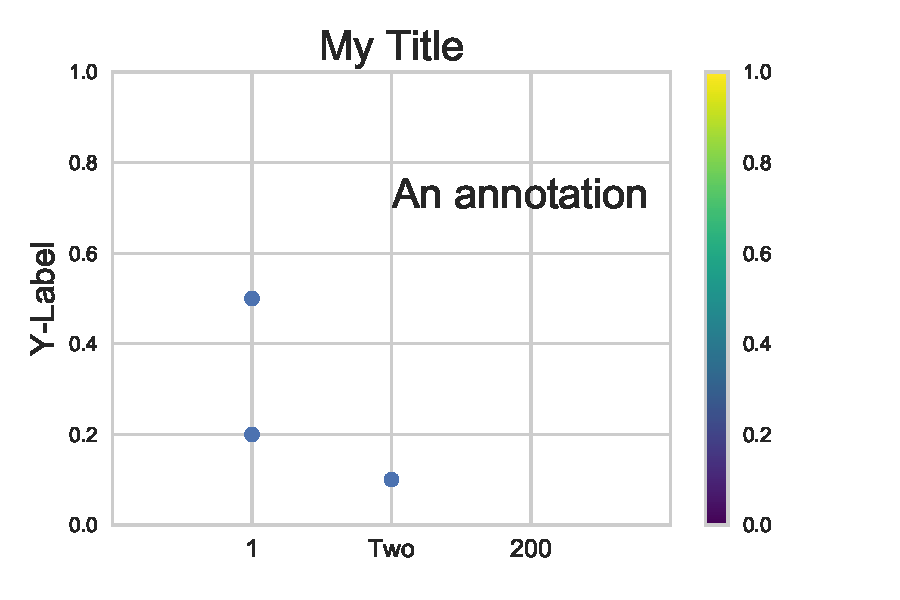
\includegraphics[width=0.3\textwidth]{../demoplot.pdf}};
\pause
\node[text=red!70!black] at (-0.2, 1.75) {\scalebox{0.8}{\tiny{\texttt{fig, ax = plt.subplots(1)}}}};
\pause
\draw[draw=red!70!black, fill=none] (-1.6, -0.3) rectangle (-1.4, 0.3); % y Label
\node[text=red!70!black] (ylab) at (-2.15, 0.07) {\scalebox{0.6}{\tiny{Axis Labels}}};
\node[text=red!70!black] (ylabcode) at (-2.15, -0.07) {\scalebox{0.6}{\tiny{\texttt{ax.set\_ylabel()}}}};
\pause
\draw[draw=red!70!black, fill=none] (-0.55, 0.8) rectangle (0.1, 1.05); % Title
\node[text=red!70!black] (title) at (-0.2, 1.35) {\scalebox{0.6}{\tiny{Title}}};
\node[text=red!70!black] (title) at (-0.2, 1.2) {\scalebox{0.6}{\tiny{\texttt{ax.set\_title()}}}};
\pause
\draw[draw=red!70!black, fill=none] (-0.8, -0.8) rectangle (0.4, -1); % x Ticks
\node[text=red!70!black] (title) at (-0.2, -1.1) {\scalebox{0.6}{\tiny{Ticks}}};
\node[text=red!70!black] (title) at (-0.2, -1.25) {\scalebox{0.6}{\tiny{\texttt{ax.set\_xticks()}}}};
\node[text=red!70!black] (title) at (-0.2, -1.4) {\scalebox{0.6}{\tiny{\texttt{ax.set\_xticklabels()}}}};
\pause
\draw[draw=red!70!black, fill=none] (0.85, -1.05) rectangle (1.2, 1.05); % Colorbar
\node[text=red!70!black] (ylab) at (1.8, 0.07) {\scalebox{0.6}{\tiny{Colorbar}}};
\node[text=red!70!black] (ylabcode) at (1.8, -0.07) {\scalebox{0.6}{\tiny{\texttt{fig.colorbar()}}}};
\pause
\draw[draw=red!70!black, fill=none] (-0.8, -0.75) rectangle (-0.1, 0.1); % Data Points
\node[text=red!70!black] (ylab) at (0.3, -0.2, 0.07) {\scalebox{0.6}{\tiny{Data Points}}};
\node[text=red!70!black] (ylabcode) at (0.3, -0.42, -0.07) {\scalebox{0.6}{\tiny{\texttt{ax.scatter()}}}};
\pause
\draw[draw=red!70!black, fill=none] (-0.3, 0.3) rectangle (0.8, 0.5); % Annotation
\node[text=red!70!black] (ylab) at (-0.7, 0.5) {\scalebox{0.6}{\tiny{Annotation}}};
\node[text=red!70!black] (ylabcode) at (-0.7, 0.3) {\scalebox{0.6}{\tiny{\texttt{ax.text()}}}};


\end{tikzpicture}

\end{document}
